% This is LLNCS.DEM the demonstration file of
% the LaTeX macro package from Springer-Verlag
% for Lecture Notes in Computer Science,
% version 2.4 for LaTeX2e as of 16. April 2010
%
\documentclass{llncs}
%
\usepackage{makeidx}  % allows for indexgeneration
\usepackage{graphicx}
\usepackage[ngerman]{babel}
\usepackage[utf8]{inputenc}
\usepackage{microtype}
\usepackage{enumitem}
%\setcounter{secnumdepth}{3}
\setcounter{tocdepth}{3}

%
\begin{document}
%
%\frontmatter          % for the preliminaries
%
\pagestyle{headings}  % switches on printing of running heads
%
%\mainmatter              % start of the contributions
%
\title{EEXCESS Redesign} 
%
\author{Mathias Möller,\\
\email{moellerm@fim.uni-passau.de}}
%
\institute{Universität Passau, 94032 Passau}

\maketitle              % typeset the title of the contribution

\pagestyle{plain}		% Zeilennummern unten Mitte


%
	%\tableofcontents
%
\section{Motivation} 
\label{sec:motivation}
Ziel dieser Arbeit ist es, ein Chrome Plugin zu entwickeln, welches, ähnlich zum EEXCESS Plugin, dem Benutzer beim Lesen einer Webseite weiterführende Quellen zum Thema der Seite vorschlägt. Dies soll es dem Nutzer ermöglichen, ohne weiteren Suchaufwand, weiterführende wissenschaftliche Quellen zu finden und so die Recherche zu vereinfachen und zu optimieren.
\newline
Während EEXCESS dem Nutzer nur Quellen zum Thema der gesamten Seite vorschlägt und diese am Rand der Browsers anzeigt, soll das neue Plugin die Paragraphen der Seite erkennen und analysieren und auf Basis dieser Informationen eine Anfrage an die Europeana-Datenbank schicken. Die Ergebnisse sollen dem Benutzer dann erkennbar zum Paragraphen gehörend angezeigt werden. Daraufhin soll der Benutzer die Möglichkeit haben, die Suchanfrage anzupassen (zum Beispiel durch Löschen/Hinzufügen von Suchwörtern).
\newline
Durch diese Änderungen im Design und Verhalten des Plugins sollen die Probleme des EEXCESS Plugins, die bei einer Nutzer-Evaluierung zu Tage gefördert wurden, behoben werden und die Usability des Programms verbessert werden.
\newline
Um dieses Ziel zu erreichen, wird die Arbeit in folgende Schritte unterteilt: Anzeige der Ergebnisse, Erklärung der Such-Anfragen Generierung, Anpassung der Suchanfrage durch den Benutzer und eventuell Ausarbeitung eines Konzepts zur automatischen Anpassung der Suchanfragen durch maschinelles Lernen.

\section{Vorarbeit}
Zu Beginn der Arbeit wird untersucht, wie die Suchanfrage an die Europeana-Datenbank aus den Paragraphen extrahiert werden kann und wie die Ergebnisse dem Benutzer dargestellt werden müssen um seine Arbeitsweise bestmöglich zu unterstützen.
\newpage

\section{Benutzeroberfläche}
Um den groben Aufbau des Plugins zu skizzieren (ohne sich auf das Design festzulegen) wurden Mockups der Benutzeroberfläche angefertigt.

\begin{figure}{}
\centering
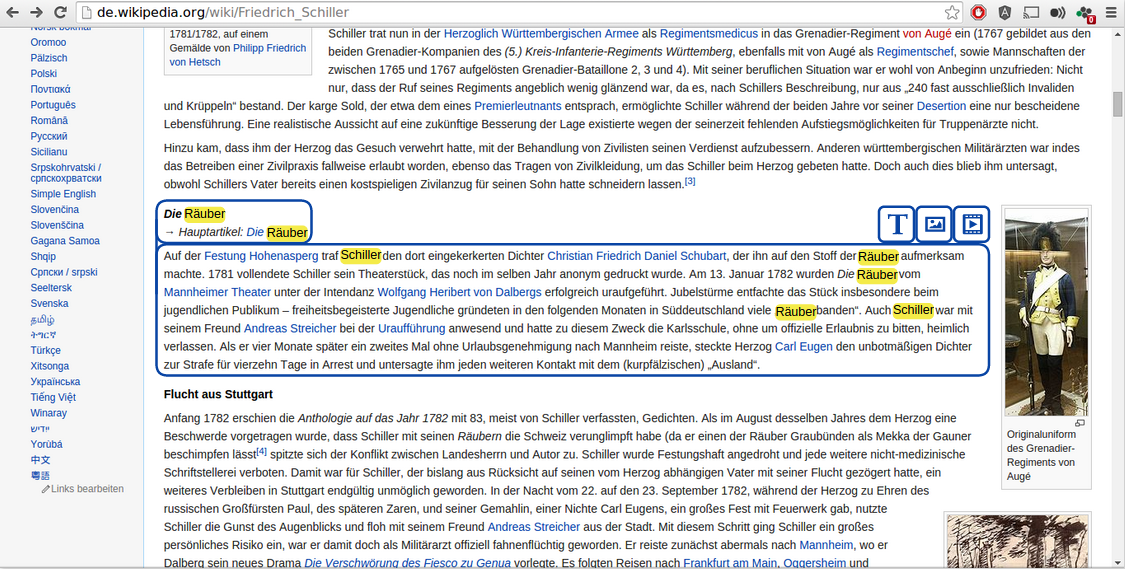
\includegraphics[height=6cm]{images/plugin_paragraph.png}
\caption{Der erkannte Paragraph wird hervorgehoben und Buttons zum Auswahl der gewünschten Quellen-Art werden angezeigt}
\label{fig:paragraph}
\end{figure}
Während des Lesens einer Webseite wird das Plugin versuchen die Paragraphen-Struktur der Seite zu erkennen. Gefundene Paragraphen werden dann hervorgehoben (siehe Abb. \ref{fig:paragraph}) und eine Analyse des Inhalts wird durchgeführt. Mit den Ergebnissen dieser Analyse wird daraufhin eine Anfrage an die Europeana-Datenbank abgeschickt. Die benutzten Suchwörter werden im Text hervorgehoben, um es dem Benutzer zu Ermöglichen, neue Suchwörter per Klick hinzuzufügen oder andere zu Löschen. 
\newline
Der Benutzer hat dann die Möglichkeit die Art der Quellen zu Bestimmen die ihm angezeigt werden sollen (siehe Abb. \ref{fig:sources}). Denkbare Auswahlmöglichkeiten wären Text-, Bild- oder Videoquellen.

\begin{figure}{}
\centering
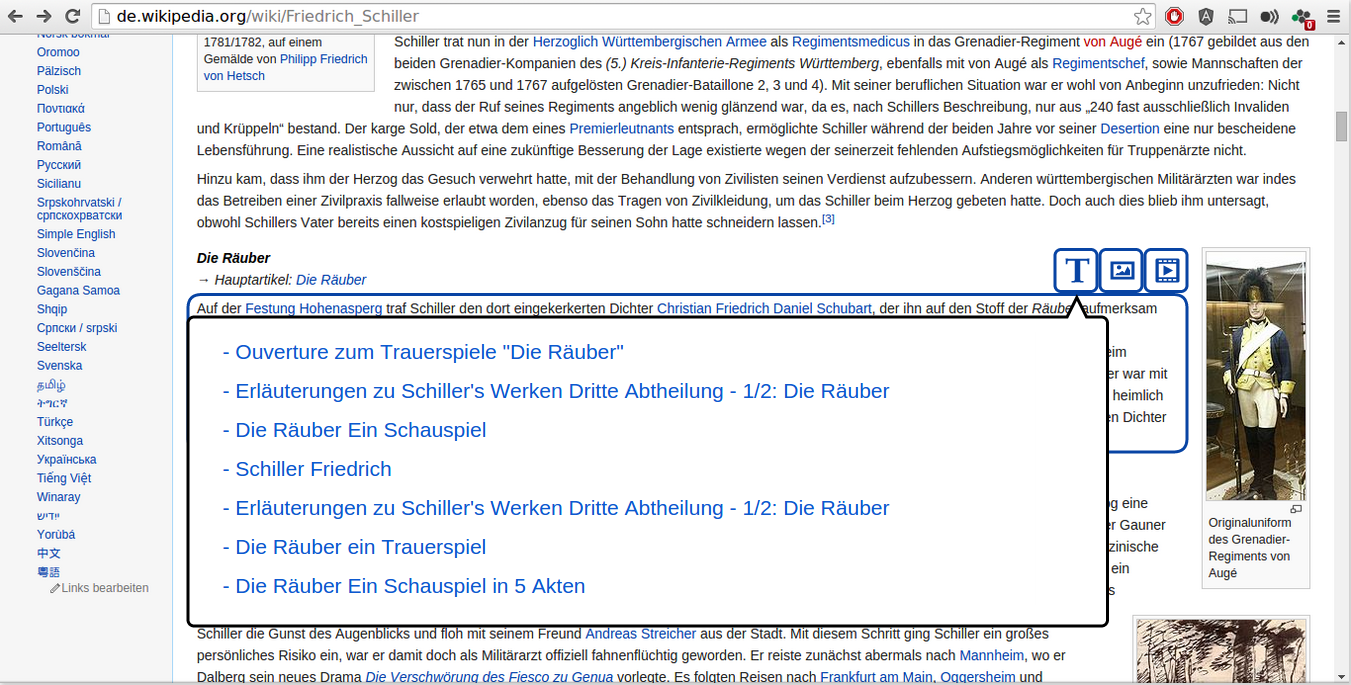
\includegraphics[height=6cm]{images/plugin_showSources.png}
\caption{Nach Auswahl der gewünschten Quellen-Art werden dem Benutzer die gefundenen Quellen angezeigt}
\label{fig:sources}
\end{figure}

\section{Verwendete Technologien}
Technologien zur Paragraphen-Erkennung sowie zur Textanalyse der Paragraphen werden vom Lehrstuhl für Medieninformatik bereitgestellt. Die Paragraphen-Erkennung wird gegebenenfalls optimiert um auch auf weniger strukturierten Seiten eine möglichst gute Erkennung zu ermöglichen.
\newline
Das Plugin wird seine Suchanfragen an die REST-API der Europeana-Datenbank schicken.

\section{Zeitlicher Ablauf der Ausarbeitung}
\begin{enumerate}[label=\Roman*)]
\item Recherche zu technischen Details der Umsetzung und Implementierung
\item Skizzieren der Programmstruktur, REST-Anfragen, Interfaces
\item Praktischer Teil:
\begin{itemize}
\item[]
\begin{description}
\item [Milestone 1:] Integration von Paragraphen-Erkennung in simples User-Interface
\item [Milestone 2:] Integration der Textanalyse und senden der Such-Anfragen an Europeana-Datenbank
\item [Milestone 3:] Anzeigen der Suchergebnisse 
\item [Milestone 4:] Manipulation der Suchanfrage
\item [Milestone 5:] Design Ausarbeitung
\item [Milestone 6:] (optional) Usability Tests
\item [Milestone 7:] Endgültiges Design 
\end{description}
\end{itemize}

\item Theoretischer Teil:
\begin{itemize}
\item[]
\begin{description}
\item [Einleitung/Motivation] Beschreibung der Motivation der Arbeit (Verbesserung des EEXCESS Plugins), Unterschiede zum EEXCESS Plugin
\item [Related Work] Vergleich des Plugins und der verwendeten Technologien (Paragraph-Erkennung, Text-Analyse) mit ähnlichen Lösungen
\item [Konzept]                                                                                           
	\begin{itemize}
		\item Allgemeines und Verweis auf 4 Unterziele
		\item Anzeige der Ergebnisse
		\item Erklärung der Such-Anfragen Generierung
		\item Anpassung der Suchanfrage durch den Nutzer
		\item Verbesserung der Suchanfrage durch maschinelles Lernen
	\end{itemize}
\item [Implementierung] Beschreibung der REST-Anfragen, der verwendeten Technologien und der Vorgehensweise während der Implementierung
\item [Evaluierung] (optional) Usability Tests mit anschließendem Vergleich mit den Ergebnissen der EEXCESS Evaluierung
\item [Future Work] Implementierung der automatischen Suchanfragen-Verbesserung durch maschinelles Lernen
\end{description}
\end{itemize}
\end{enumerate}
% section zeitlicher_ablauf (end)

\end{document}